\section{Introduction}
The field of artificial intelligence (AI) has been extremely popular over recent years, due to the wide range of applications the technology has developed with the help of modern computer hardware. Machine learning algorithms are capable of outperforming humans at a variety of different tasks while being significantly faster and cheaper to operate. Possible applications include self-driving vehicles, computer-aided interpretation of medical imagery, stock market analysis, and robotics. However, despite their sometimes impeccable performance, current artificially-intelligent programs have a common drawback, which is their inability to generalize to other tasks. Each algorithm is developed by human experts specifically to solve a single problem and is hence referred to as \textit{artificial narrow intelligence}. A program capable of learning many different tasks, similar to a human, is called \textit{artificial general intelligence} (\textit{AGI}), and developing such a program is the holy grail of AI research.

Learning systems can be subdivided into three categories, namely \textit{supervised learning}, \textit{reinforcement learning}, and \textit{unsupervised learning}. In supervised learning, the learner is presented with examples of input-output combinations, for which it must adopt a mapping that generalizes well to previously unseen inputs. For some problems, however, no sufficient number of examples that include their respective solutions (or outputs) exist, making supervised learning intractable. Consider the movement of a bipedal robot. Gathering a large set of training examples on how to walk for a variety of different scenarios for a learning system would require an already existing solution to the problem we are trying to solve. It is, however, relatively trivial to judge the robot's performance. For instance, the act of falling over is easy to detect and clearly undesirable, whereas a steady forwards movement should be encouraged. Learning, that is only based on this feedback, is called reinforcement learning. The final category, unsupervised learning, is used for data in which neither a perfect solution nor a rating (as in the former categories) is available. These algorithms try to structure data by finding hidden patterns or similarities, which may, for example, be used in data visualizations.

While supervised learning is widely applicable and even considered somewhat solved by some people, reinforcement learning is still in its infancy. This is not due to an absence of use cases, however. A grasping motion of a robotic arm works well with a pre-written script in a factory setting but requires a learning system to deal with the disorderliness of the real world. Despite remarkable strides being made in recent times, with reinforcement learning algorithms playing complex board and video games at a superhuman level, \textit{sample efficiency}, the effectiveness with which the algorithm learns from few training examples, continues to be a big issue. Sample efficiency is especially critical in the field of robotics, as real-world training is costly and throttled by physical limitations, whereas simulations are computationally expensive and inaccurate.

Reinforcement learning algorithms are further classified into two groups. There are \textit{model-free} algorithms, which can be viewed as behaving instinctively, and \textit{model-based} algorithms, which can plan their next moves ahead of time. The latter is arguably more human-like and has the added advantage of being comparatively sample efficient. Furthermore, it is clear why a robot interacting with an environment, for instance, by catching a ball, would benefit from anticipating the behavior of other objects within its vicinity, especially when we consider the delay between sensory information arriving and its motors being actuated.

The \textit{MuZero Algorithm} \cite{muzero} has made recent breakthroughs by becoming the new state-of-the-art model-based reinforcement learning algorithm. It outperforms its competitors in a variety of tasks, while simultaneously being very sample efficient. This makes it appear to be a fairly general-purpose algorithm and an excellent candidate for our experiments involving robot grasping (see Figure \ref{fig:cube_stacking}).
\begin{figure}[tb]
    \centering
    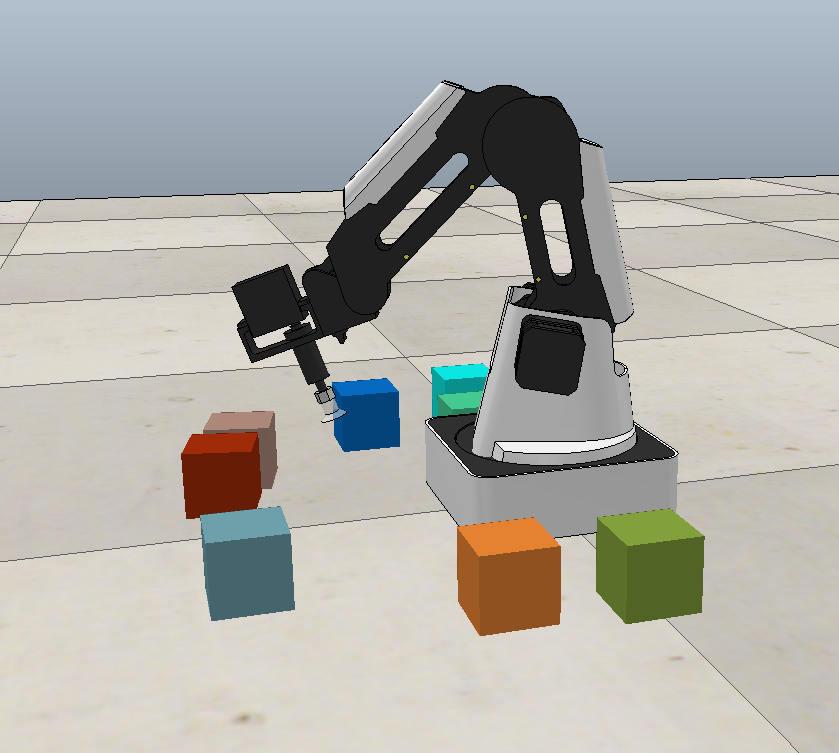
\includegraphics[width=0.5\textwidth]{assets/cube_stacking.png}
    \caption{A \textit{Dobot} robotic arm being tasked with picking up and stacking simulated cubes in \textit{CoppeliaSim} (\url{https://www.coppeliarobotics.com/}).}
    \label{fig:cube_stacking}
\end{figure}

Unfortunately, upon further investigation, we realized that MuZero performed relatively poorly on our robot experiments and was slow to operate. Contrary to our expectations, older, model-free algorithms such as \textit{A3C} \cite{a3c} delivered significantly better results while being more lightweight and comparatively easy to implement. Even in very basic tasks, our custom implementation as well as one provided by other researchers, \textit{muzero-general} \cite{muzero-general}, produced unsatisfactory outcomes.

Since this contradicts the results provided in the MuZero publication, we are led to believe that MuZero may require a team of experts and expensive hardware to reach its full potential. We question some of the design decisions made for MuZero and attempt to make it more approachable for simpler tasks.